\chapter{Spoken dialogue systems and incremental processing}
\label{ch:soadialogue}

\section{Human dialogue}
\subsection{Dialogue acts}
    \label{soa:dialogueacts}
    
    If I say \textit{This dog is big}, I utter a few sounds that can be cast as words. How are these words related to the real objects I refer to? How comes that a sequence of sounds can have effects on others? I can give orders to somebody and make them performs the actions I want as I can congratulate or insult someone and have an emotional impact on her. Also, how comes an utterance can also be judged as a complete nonsense or as a true or false assertion? These are a few questions raised in the philosophy of language.
    
    In his book called \textit{How To Do Things With Words} \cite{Austin1962}, J.L. Austin focuses on the concept of \textit{speech act}, the title of another book \cite{Searle1969} by John R. Searle, who completed this theory of language. Introducing these concepts is aimed towards bringing answers to the previous questions. Saying \textit{My sister just arrived}, one performs a speech act that can be viewed from different points of view. Suppose that someone is listening as this sentence is being uttered and that person does not speak English, then obviously she only hears a sequence of noises which is the physical, low-level nature of the speech act. When considered from that perspective, the latter is referred to as a \textit{phonetic act}. These sounds can then be put together to form a set of vocables and words which constitute a \textit{phatic act}. When the whole meaning of the sentence is taken into account, the speech act is said to be a \textit{rhetic act}. These three levels of analysis are grouped into a bigger concept, the \textit{locutionary act}.
    
    When one focuses not only on the raw meaning of a speech act but on the message that it contains, whether it is a warning or an encouragement for example, it is said to be an \textit{illocutionary act} as beyond the rhetic aspect, an \textit{illocutionary force} is considered. Nevertheless, in \cite{Searle1968}, Searle rejects this distinction between the rhetic and the illocutionary act made by Austin. According to him, the limit between the two is not justified hence rejecting the whole \textit{locutionary act} concept. Instead, he suggests to adopt a modified classification. These considerations are, however, beyond the scope of this thesis as the philosophy of language will only be used as a tool to better analyse turn-taking phenomena (see chapter \ref{ch:taxonomy}). Therefore, only two concepts will be retained: the phonetic act where the speech act is viewed as a succession of sounds and the \textit{illocutionary act} where the meaning is taken into account.
    
    Moreover, saying something to somebody can have psychological effects on that person: congratulating someone or insulting him can be rewarding or hurting, a strongly grounded speech can be convincing, etc. These are referred to as \textit{perlocutionary acts}.
    
    To build a dialogue system, the traditional approach is to consider the user's and the system's speech acts as illocutionary (and sometimes perlocutionary) acts. When studying incremental dialogue systems, the \textit{phonetic act} point of view comes into play. In this thesis, this distinction will be clarified.
    
    In the field of psycholinguistics, Herbert H. Clark brings another vision of dialogue acts in his book \textit{Using Language} \cite{Clark1996}. The communication channel is split into two tracks, the \textit{communication track} and the \textit{meta-communication track}. The first one is used when the speaker adds new information about the topic of the information whereas the second one is used when she refers to the dialogue itself. For example, saying \textit{OK, I see} or nodding her head are meta-communicative acts. 
        
    In order to guide the user throughout the dialogue, correct potential errors and to confirm some pieces of information, spoken dialogue systems use the meta-communica-tion track. In this thesis, it is shown that incremental dialogue opens new possibilities to make an even more subtle use of this track.
        
    \subsection{Turn-taking in human dialogue}
    \label{soa:ttphuman}
    
    Turn-taking is a sociological phenomenon that has been generalised to many different situations: card games, road traffic regulation, CPU resource sharing... The term \textit{turn-taking} has been applied in that context for the first time both in \cite{Yngve1970} and in Ervin Goffman's personal communications (June 5$^{th}$ 1970) independently. \cite{Duncan1972} notices that \textit{beyond considerations of etiquette, it is difficult to maintain adequate mutual comprehensibility when participants in a conversation are talking at the same time}. In \cite{Sacks1974}, Harvey Sacks describes the social organisation of turn-taking as an economy where \textit{turns are valued, sought or avoided}, depending on the situation at hand. Then, in the rest of his paper, he focuses on the case of human conversation. Obviously, this is subject to many contextual and cultural variations but the goal of the paper is to meet the challenge of extracting a set of rules that would ultimately describe the human turn-taking mechanisms in a general fashion.
        
        For about six years, Harvey Sacks has been analysing conversation recordings and he came up with a few rules that caracterise human conversation and turn-taking. One of them is particularly interesting given the purpose of this thesis: \textit{Transition (from one turn to a next) with no gap and no overlap are common. Together with transitions characterized by slight gap or slight overlap, they make up the vast majority of transitions}.
        
        In fact, this principle has been brought to light even earlier in \cite{Sullivan1947} where it has been noticed that the same turn-taking phenomena still hold over most of the languages. \citet{Schegloff1968} suggests that speaking \textit{one party at a time} is one of the basic rules for conversations. Nevertheless, when analysing human conversation more closely, it is shown that humans interrupt each other very frequently \cite{Beattie1982,Strombergsson2013}. In this thesis, this idea is extended to human-machine dialogue and it is shown that it might be interesting to interrupt the speaker in some cases in order to increase dialogue efficiency.
        
        During the following decades, a few other attempts to come up with models and classification of turn-taking phenomena in human dialogue have been made. In \cite{Beattie1982}, a political interview between Margaret Thatcher and Jim Callaghan has been analysed. As a result, the author introduced a classification of turn-taking phenomena where each category is characterised by the answer to these three questions (resulting in a general categorisation with five broad classes):
        
        \begin{enumerate}
            \item Is the attempted speaker switch successful?
            \item Is there simultaneous speech?
            \item Is the first speaker's utterance complete?
        \end{enumerate}
        
        If the listener manages to successfully take the floor and there is simultaneous speech present, either the speaker's utterance is complete which leads to an OVERLAP or not which translates into a SIMPLE INTERRUPTION. On the contrary, if there is no simultaneous speech, either the speaker's utterance is complete which leads to a SMOOTH SPEAKER SWITCH, either a SILENT INTERRUPTION is involved. Finally, if the listener does not succeed in taking the floor, only one category is reported: BUTTING-IN INTERRUPTION. In \cite{Gravano2011}, this classification is extended by introducing the following question: \textit{Is the listener's utterance in response to the speaker's one and indicates only ``I am still here/I hear you and please continue?''}. As a consequence, two new categories are introduced when the answer is yes and given the fact that there is simultaneous speech or not: BACKCHANNEL and BACKCHANNEL WITH OVERLAP.
        
        Optimising turn-taking means taking the floor at the right time. Humans are very good at detecting the cues for these timings \cite{Raux2008,Jonsdottir2008,Gravano2011}: prosodic features, lexical features, semantic features, ...

        Actually, humans even tend to start speaking before the end of their interlocutor's utterance, even interrupting him sometimes. A study led in \cite{Strombergsson2013} reports statistics about times and overlaps in human conversation both directly and over the telephone. Given the type of question that is addressed to the listener, the latter tends to respond more or less quickly, often inferring the end of the question and starts uttering the response before its end.
        
        In reality, human turn-taking involves even more complicated behaviours resulting in intertwined turns between the speakers. \citet{Raux2009} tries to provide a simple model with very few assumptions. It is a state machine where the following states are considered (initially depicted in \cite{Jaffe1970}):

        \begin{itemize}
          \item Only the user speaks.
          \item Only the system speaks.
          \item No one speaks because the user stopped talking.
          \item No one speaks because the system stopped talking.
          \item Both the user and the system speak after a user barge-in.
          \item Both the system and the user speak after a system barge-in.
        \end{itemize}
        
        In this framework, four basic turn-taking transitions are introduced: \textit{turn transitions with gap}, \textit{turn transitions with overlap}, \textit{failed interruptions} and \textit{time outs}. This is a very low-level model where only phonetic acts are considered (unlike the classification proposed in \cite{Beattie1982} for example where the intent of the listener when he tries to take the floor is taken into account). A similar approach is used in \cite{Wlodarczak2013}, but the situations identified are different:

        \begin{itemize}
           \item \textbf{Within-speaker silence:} The speaker stops for a while and then resumes his utterance.
           \item \textbf{Between-speaker silence:} The most intuitive case of turn taking. The speaker stops and after a moment of silence, the listener takes the floor.
           \item \textbf{Within-speaker overlap:} The listener either takes the floor or performs an intervention that is not meant to interrupt the speaker and the latter keeps the floor.
           \item \textbf{Between-speaker overlap:} The listener starts speaking before the end of the speaker's utterance, hence resulting in an overlap and a turn transition.
           \item \textbf{Solo vocalisation:} On person speaks in an unilateral way.
        \end{itemize}
        
        \subsection{Incremental speech processing in human dialogue}
        \label{soa:inchuman}

           During a conversation, the listener does not wait for the speaker's utterance to end before trying to understand it. It is processed incrementally and on top of the intuition that people have related to this, a few studies provided convincing arguments supporting the idea. The most famous and convincing examples are eye-tracking based studies \cite{Tanenhaus1995,Eberhard1995,Arnold2000}. Subjects are given an image to look at through a head-mounted eye-tracking mechanism that records their eye-gaze at a millisecond scale. Then, ambiguous and unambiguous sentences were uttered, for example:

           \begin{itemize}
             \item \textbf{Ambiguous version:} Put the apple on the towel in the box.
             \item \textbf{Unambiguous version:} Put the apple that is on the towel in the box.
           \end{itemize}

           For this example, when the users are provided with an image of an apple on a towel, a towel with nothing on it and a box, their eye-gaze shows different patterns depending on which version of the utterance they listen to. In the ambiguous case, they tend to start by looking at the apple, then to the towel with nothing on it, then to the apple again and finally at the box. In the unambiguous case, they directly look at the apple and then to the box. Most importantly, these movements happen as the sentence is uttered.

           This is also pretty much related to the garden path sentence effect. Consider the following sentence (taken from the related Wikipedia article): \textit{the government plans to raise taxes were defeated}. Most people feel the need to read it twice or even several times before understanding its meaning. When one starts reading \textit{the government plans to raise taxes}, she automatically understands that taxes are planned to be raised by the government but then comes the disturbing end of the sentence: \textit{were defeated}. The only solution is to parse \textit{plans} as a noun and not as a verb. This is also an argument in favour of human incremental processing.

           Finally, when humans are reading a text, they tend to skip a few words with no loss of the meaning. In \cite{Ilkin2011}, the authors show that it is possible to predict a few words while reading given the context and the sentence structure (eye-tracking has also been used here). For example, when the readers reach the sentence \textit{The worker was criticised by his boss}, the word boss seems to be guessed ahead of time, again supporting the idea of incremental processing.


\section{Spoken dialogue systems}
        
A spoken dialogue system (SDS) is an automated application that interacts directly with a human being in natural language. Virtual assistants like Siri (Apple) or Cortana (Microsoft) are good examples of SDSs. They are task-oriented since their goal is to help the user achieve some task. There also exist a few SDSs that are only used for tutoring \cite{Jordan2015} or simply chatting and companionship \cite{Sidner2013}.

Historically, McCarthy and Hayes were the first to suggest the introduction of mental qualities (intentions, belief, ...) in a dialogue system \cite{McCarthy1969,McCarthy1979} in the 70's. This started a new research thread aimed at describing the internal state and the system's behaviour in a humanlike fashion \cite{Newell1980,Bratman1987,Cohen1990,Sadek1991,Konolige1993}. In Orange, a new dialogue system called ARTIMIS has been developed. It was based on a new theory of interaction \cite{Sadek1991} using the Belief-Desire-Intentions model introduced in \cite{Bratman1988}. During the following years it has been improved and enhanced with new capabilities: an action plan \cite{Louis2002}, a preference-based operator \cite{Meyer2006} and uncertainty management capacities \cite{Laroche2008}.

However, this approach that uses logic has been abandoned for two main reasons. Firstly, it does not guarantee the VUI-completeness \cite{Pieraccini2005,Paek2008}: it can lead to system behaviours that have not been specified in advance by the designer, and secondly it requires an expertise in the logic field (which considerably reduces the span of potential dialogue system designers). As a result, like all the major actors in the field (Nuance, AT\&T, SpeechCycle, etc.), Orange turned to a new solution where the dialogue system is viewed as an automaton. This solution is called Disserto which has proved to be simple, robust enough to allow the development of widely deployed industrial dialogue systems and flexible enough to allow state-of-the-art research. All the services developed in this thesis have been generated using Disserto which will be presented more deeply later on.

\subsection{Towards a human-like interaction}
  \label{soa:humanlike}
  
  Traditional computer interfaces are presented in the form of controls in an application (text boxes, buttons) or web pages. They are heavily used and they have been proven to be efficient enough, providing an accurate way of human-machine interaction. So, why building spoken dialogue systems? What are the advantages of the vocal modality?
  
  An obvious motivation for building spoken dialogue systems is the quest for human-likeness. In \cite{Edlund2008}, an interesting analysis of the way humans perceive dialogue systems they are interacting with is performed. These systems are complex and humans keep a biased representation of them during the interaction (called metaphors in the article). Two of them are the most common:
  
  \begin{itemize}
    \item \textit{Interface metaphor:} The system is viewed as an interface just like non dialogue-based systems. Users adopting this representation of the system tend to use vocal commands instead of complete sentences. Moreover, they tend to remain silent when the system tries to behave like a human, by saying \textit{Hi!} for example.
      \item \textit{Human metaphor:} In this case, the users tend to view the system as a real human, therefore adopting a more natural way of communication. These users generally have higher expectations of the system's ability to answer their requests as well as its ability to perform human-like turn-taking behaviours.
        \end{itemize}
        
        Nevertheless, it is also legitimate to raise the question whether human-likeness should be a goal in the conception of dialogue systems or not. In \cite{Edlund2008}, four kinds of objections to pursuing that goal are discussed. The first one is the feasibility: is there any hope that someday, systems that behave exactly like humans could be built? This has raised huge debates during the last decades. The second question is utility: do people really need systems that imitate humans? Apart from the fact that it would help us to better understand the way humans communicate, it is an interesting application in the case of some applications like companionship and entertainment. It is less obvious when it comes to task-oriented dialogue. The third point is related to the concept of \textit{uncanny valley} \cite{Mori1970}: as machine's human-likeness increases, they reach a point where they start behaving like humans without having the same capacities which makes them disturbing for the user. The reason behind that is the concept of symmetry (last brought up question in the paper): if machines have a similar behaviour to humans, then users are likely to push the human metaphor to the limit by unconsciously thinking that machines really understand what they are saying, thus expecting more complex reactions like the ones due to emotions for example. Nevertheless, by bringing even more improvements, this valley will be hopefully crossed and human-like solutions that no longer have such problems will be built.

        The multiplication of services and support platforms in modern society engenders huge costs that dialogue systems can help to reduce. By analysing client paths while requiring assistance from an expert, it is possible to identify commonly asked questions and recurrent patterns. By gathering such information, it is also possible to design dialogue systems that can interact with users and respond to their requests without any human intervention (of course, in the case the interaction fails, the client is redirected to a human-operated service platform). This can dramatically reduce service and support costs and also improve the quality of service as it is accessible any time, with no interruptions (unlike real platforms that are more often open at working time only). Moreover, when a client calls, the answer is immediate and her call is no longer queued causing waiting time (which she may pay for) with sometimes no answer in the end.

        With the development of the IoT during the last few years, new human-machine interactions can be imagined. For instance, the concept of \textit{Smart Home} is currently making its entry in the market of Artificial Intelligence through the contributions of several companies and start-ups: Amazon Echo, etc. In this context, the advantage of speech communication is clearly relevant as it is hands- and eyes-free. The user can command her house from any room with no extra device needed. In some situations, her hands are already occupied by some other task. For example, she can be cooking \cite{Laroche2013} while asking \textit{What should I put next in my salad?} or \textit{Can you add milk to my shopping list please?}.

        Finally, as talking agents and talking robots can also be designed for entertainment and companionship \cite{Gelin2010,Sidner2013} and the vocal modality is the most natural way of interaction, it is very useful in this area.
        
        \subsection{Spoken dialogue systems architecture}
        \label{soa:architecture}

        
        \begin{figure}
          \centering
          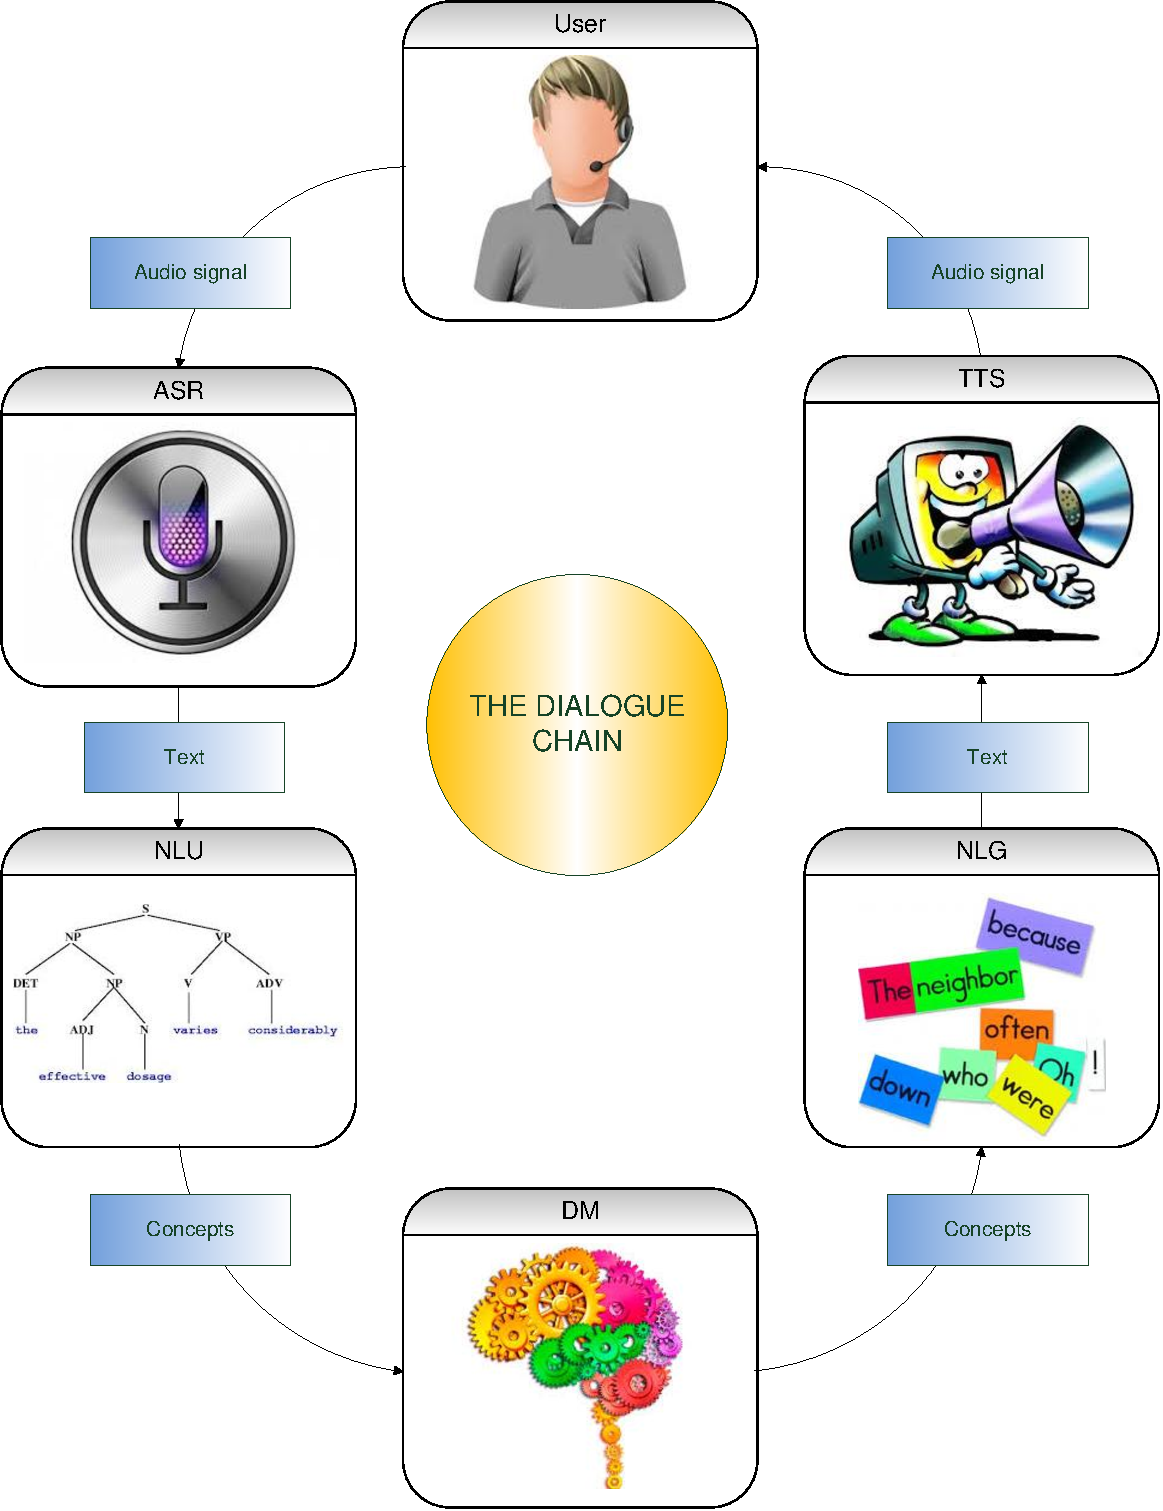
\includegraphics[scale=0.8]{figures/DialogueChain.pdf}
          \caption{The dialogue chain}
          \label{fig:dialchain}
          \end{figure}

          The classic architecture of an SDS is made of five main modules (Figure \ref{fig:dialchain}):
          \begin{enumerate}
            \item Automatic Speech Recognition (ASR): transforms the user's audio speech signal into text.
              \item Natural Language Understanding (NLU): outputs a conceptual representation of the user's utterance in text format.
                \item Dialogue Manager (DM): given the concepts extracted from the user's request, a response (in a conceptual format too) is computed.
                  \item Natural Language Generation (NLG): transforms the concepts computed by the DM into text.
                    \item Text-To-Speech (TTS): reads the text outputted by the NLG by using a synthetic voice.
                      \end{enumerate}
                      
                      \subsubsection{Automatic Speech Recognition}

                      %HK> Rajouter des références.
                      Speech recognition technology is an old problem with long history. During the 1950s, a group of researchers from Bell Labs developed the first technology that was able to recognise digits from speech (in fact, speech perception has been under study since the early 1930s). Then, during the second half of the last century, new advances have made it possible to build ASR solutions with larger vocabulary and with no dependence on the user. In the 1960s, Hidden Markov Models (HMMs) were proved to be useful for speech recognition \cite{Gales2007} and they were the most popular technique two decades later. Commercial products using ASR technology had to wait until the 1990s to be finally released in the market as they reached an interesting vocabulary scope (even though their accuracy and their delay were far behind the technology available today). Performances kept improving slowly and gradually until 2009, when Deep Learning algorithms were tested \cite{Mohamed2009,Deng2013} introducing huge improvement; the Word Error Rate (WER) decreased by 30\%. During the last six years, research continued in that direction giving birth to accurate and reactive speech recognition solutions (Google, Nuance, Sphinx, Kaldi...). These solutions also provide results incrementally in a continuous fashion. Therefore, ASR is less and less considered as a bottleneck in the development of spoken dialogue systems, and as it will be shown later, the delays they offer make it possible to design reactive incremental dialogue systems. Commercial off-the-shelf ASR solutions like Google ASR or Nuance products are able to recognise almost every word in many languages, including named entities. Finally, the ASR output is not only the text that the recognition algorithm figures out to be the best match for the input audio signal, but a list of the N most likely hypotheses and the corresponding confidence scores: it is called the N-Best. For instance, a 5-Best example is represented in Fig. \ref{fig:fivebest}.
                      
                      \begin{figure}
                        \centering
                        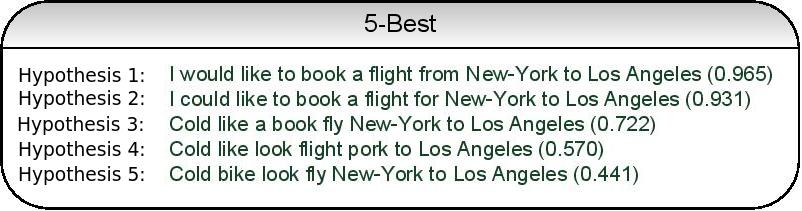
\includegraphics[scale=1]{figures/5BestEx.jpg}
                        \caption{A 5-Best example corresponding to the sentence ``I would like to book a flight from New-York to Los Angeles''.}
                        \label{fig:fivebest}
                        \end{figure}
                        
                        \subsubsection{Natural Language Understanding}
                        
                        NLU is a sub-field of Natural Language Processing (NLP) which scope is wider than the spoken dialogue field. Since the 1950s, researchers have been trying to develop several models and ontologies in order to automatically process natural language with several applications in sight: topic recognition, sentiment analysis, news filtering and analysis, natural speech processing, etc. The ambition manifested during the 1950s and the early 1960s quickly had to face reality as the expected objectives were far from being reached. As a consequence, research in this area was significantly slowed down between the 1960s and the 1980s. During the last decade, NLP research has found a second wind thanks to new Machine Learning techniques, bringing them at the heart of lucrative businesses like recommendation and digital marketing. NLU refers to the set of techniques in order to make the machine understand the underlying structure of a text in natural language. To do so, a lexicon as well as an ontology (concepts and the links between them in a specific domain) should be built. Therefore, earlier NLU solutions are based on a set of handcrafted parsing rules, however, new statistical-based models \cite{Macherey2009,Hahn2010} have been proven to be more robust and easy to generalise over domains. Also Deep Learning has also been applied to NLP showing interesting performances that NLU modules can benefit from \cite{Bengio2003,Collobert2011,Ferreira2015a,Ferreira2015b,Ferreira2016}.

                        \subsubsection{Dialogue Management}
                        
                        As far as Dialogue Management is concerned, two decades ago, for the first time, dialogue has been modeled as Markov Decision Processes (MDPs) problem (see Sect. \ref{soa:rl}), hence being solved using reinforcement learning \cite{Levin1997a}. The dialogue state contains all the information needed to determine what is the best action to perform as well as the quality of that state (roughly speaking, to what extent it is desirable for the system to be in that state). The possible actions in each state are the dialogue acts that the system can make while being in that state. In 2007, in order to represent the uncertainty over the user's intent (due to ASR or NLU imperfections), dialogues have been cast as Partially Observable Markov Decision Processes (POMDPs) \cite{Roy2000,Williams2007}. This gave raise to the notion of \textit{belief tracking} which objective is to keep a distribution over the possible user intents. Also, existing dialogue systems are able to interact with the user in the domain they are built for only, however, during the last few years, researchers have been pushing the boundaries of domain  extension methods \cite{Gasic2013} and open-domain systems \cite{Pakucs2003,Galibert2005,EkeinhorKomi2014,Wang2014}. Finally, it has been shown that it is possible to use reinforcement learning to continously adapt to users online \cite{Ferreira2015c,Chandramohan2012a,Chandramohan2012b}.
                        
                        \subsubsection{Natural Language Generation}
                        
                        The NLG task is the inverse of the NLU one: it translates dialogue acts concepts into sentences. It started being used in the 1990s for purposes like business and financial news summary \cite{Anand1992}. A few start-ups and big companies also provide automatic text generation solutions that are used to quickly produce reports or official letters. The main challenge for such systems is to be able to generate a variety of different words, expressions and sentences in order for them not to be repetitive and for the result to be as realistic as possible. This is even more crucial when it comes to dialogue systems as they are supposed to simulate real conversations with the user, which is a highly variable. Nevertheless, in practice, template-based generation methods are the most widely used even though data-driven solutions are starting to reach mature development \cite{Mairesse2010,Mitchell2014,Manishina2016}.
                        
                        \subsubsection{Speech Synthesis}

                        During the 1930s, Bell Labs were not only interested in ASR but they also developed a new approach for the reciprocal task: the TTS (also known as \textit{speech synthesis}). The human speech is broken into small acoustic components that are sequentially pronounced by the system. They built the first machine demonstrating this mechanism: the Voder \cite{Dudley1939}. As far as this task is concerned, the challenge for the system is to sound as human-like as possible, in terms of phoneme transitions, speech rate and prosody. Two research threads tackle this problem in two different manners \cite{Tabet2011}: the first one uses corpus-based methods where the resulting audio is a combination of pre-recorded phonemes extracted from a corpus and the second one uses HMMs to generate a completely synthetic voice. Even though substantial advances have been accomplished since the Voder, including data-driven approaches \cite{Yu2011}, it is still easy to distinguish between a synthesised and a real human voice.

                        \subsection{Spoken dialogue systems evaluation}

                        When building dialogue systems and improving them, it is necessary to determine metrics in order to measure their evolution. What makes a dialogue system better than another one? What metrics should be taken into account while evaluating dialogue systems? What are the most important characteristics of a dialogue system that should be improved?
                        
                        A distinction can be made between the evaluation of a dialogue system as a whole (\textit{usability} as it is called in \cite{Moller2007}) and the evaluation of the different components separately. In the second case, more standard metrics exist such as the Word Error Rate (WER) for the ASR or the CER (Concept Error Rate) when it comes to evaluating the NLU. However, all errors are treated the same whereas in reality, some of them have more impact than others. This is a complex problem since even humans disagree when it comes to assessing the \textit{gravity} of each error \cite{Rosset2013}. Also, as far as the DM is concerned, such metrics do not exist: the usability evaluation is preferred to a local evaluation of the DM since they are very correlated \cite{Dybkjaer2004}. As a consequence, many evaluation frameworks for dialogue systems have been developed and used both in academia \cite{Walker1997,Hone2000,Schmitt2012} and industry \cite{Evanini2008,Witt2011}.

                        In the evaluation literature, a distinction is made between two kinds of metrics that are usually used for evaluating dialogue systems: objective and subjective metrics. The first category contains all the Key Performance Indicators (KPIs) that can be measured by an algorithm by accessing the dialogue information and meta-information, whereas the second one is made of the user's appreciations of the dialogue quality or specific characteristics like human-likeness or to what extent the user enjoyed the dialogue experience.

                        Objective metrics that are commonly used are the dialogues' mean duration and the task completion ratio. Generally speaking, these two metrics are correlated as the user gets impatient when the dialogue lasts for too long (the user can also get impatient for other reasons, like the repetition of the same system's dialogue act several times). Moreover, the user's speech rate and the way they communicate introduces some variability when using these metrics. Finally, it is legitimate to ask the question: are shorter dialogues the real desired objective? First, this depends on the type of dialogue system at hand. If it is designed for entertainment or companionship, then there is no need for seeking faster dialogue strategies. However, in the case of task-oriented dialogue, looking for shorter dialogues makes sense as a measure of efficiency. In these situations and especially for daily tasks, an efficiency threshold has to be necessarily reached in order for people to use the dialogue system at hand.

                        Subjective metrics are generally gathered using a survey at the end of each dialogue or by making experts rate dialogues afterwards. Several metrics can be collected this way: the global quality of the dialogue, naturalness/human-likeness, reactivity, etc. However, this also raises the problem of variability between users. Most often, they are asked to evaluate the system on a Likert scale (1 to 5 or 1 to 10), but a user answering 4 could be equivalent to another user answering 3 or 5. Therefore, the absolute evaluation is less significant than the relative one given a specific user.


\section{Incremental dialogue systems}

\subsection{Principles}

    Most dialogue systems have a simple and rigid way of managing turn-taking. The interaction mode they offer is similar to a walkie-talkie conversation as the system waits for the user to finish her utterance before taking the floor and vice-versa (even though some systems allow the user to interrupt them). Such systems will be referred to as \textit{traditional dialogue systems} in this thesis.
    
    The first idea of incremental systems goes back to incremental compilers \cite{Lock1965}. An incremental compiler processes each new instruction independently from the previous ones. Therefore, a local modification of the code does not affect the whole result of the compilation. The idea of processing natural language in an incremental way is first introduced in \cite{Wiren1992} according to \cite{Kilger1995}. Instead of feeding modules with complete utterances, the input is pushed chunk by chunk (500ms of audio signal, one word of a sentence...etc...) making the output change several times before the end of the user's utterance. Nevertheless, in his book \textit{Speaking: From Intention to Articulation} \cite{Levelt1989}, Levelt analysed the mechanisms underlying the way humans formulate their ideas in natural language and already reported that the processes involved are incremental. The approach is closer to computational linguistics than psycholinguistics. The second part of the dialogue chain (DM, NLG and TTS) is analysed using a different terminology: the \textit{Conceptualizer}, the \textit{Formulator} and the \textit{Articulator}.

    As discussed in Sect. \ref{soa:inchuman}, in human-human conversation, the listener does not wait for the speaker to finish his sentence before processing it; it processes it as it is spoken. As a consequence, human beings perform a large panel of turn-taking behaviours while speaking, like backchanneling (\textit{aha}, \textit{yeah}, ...) or barging-in.

    To replicate these behaviours, a new generation of SDSs has been the focus of research for the last few years. An SDS is said to be incremental when it is able to process the user's speech on the fly. The input signal is divided into small chunks and the growing sentence is reprocessed at each new chunk \cite{Schlangen2011}. Table \ref{tab:incrnluex} gives an example illustrating the functioning of an incremental NLU module (in a hotel room booking service). For the sake of simplicity, processing delays are neglected.

    \begin{table}[th]
      \vspace{2mm}
      \centerline{
        \begin{tabular}{|l|l|l|}
          \hline
          \textbf{Time step} & \textbf{NLU input} & \textbf{NLU output} \\
          \hline
          1 & I & empty \\
          \hline
          2 & I won't & empty \\
          \hline
          3 & I would & empty \\
          \hline
          4 & I would like to & empty \\
          \hline
          5 & I would like to cook a & empty \\
          \hline
          6 & I would like to book a room & \textbf{action:} BOOK \\
          \hline
          7 & I would like to book a room on May & \textbf{action:} BOOK \\
          \hline
          8 & I would like to book a room on May 7$^{th}$ & \textbf{action:} BOOK \\
                             & & \textbf{date:} 05-07 \\
          \hline
          9 & I would like to book a room on May 17$^{th}$ & \textbf{action:} BOOK \\
                             & & \textbf{date:} 05-17 \\
          \hline
          10 & I would like to book a room on May 17$^{th}$ and I will & \textbf{action:} BOOK \\
                             & & \textbf{date:} 05-17 \\
          \hline
          11 & I would like to book a room on May 17$^{th}$ and I will & \textbf{action:} BOOK \\
                             & be driving & \textbf{date:} 05-17 \\
                             & & \textbf{parking:} YES \\
          \hline
        \end{tabular}
      }
      \caption{Example of incremental NLU processing}
      \label{tab:incrnluex}
    \end{table}

    \newpage

    This mechanism allows the system to react earlier, even before the end of the user's utterance. On the other hand, allowing the user to interrupt the system does not require incremental capabilities; it has been successfully implemented in non-incremental dialogue systems \cite{Lamel2000,El-Asri2014a}.

      \subsection{Advantages of incremental processing}

                Before discussing the different reasons why incremental processing should be preferred to rigid turn-taking, it is important to note that a few studies with real users have shown that incremental dialogue systems offer a better user experience. For instance, in \cite{Aist2007}, an ordinal regression has been performed between the user satisfaction and several features with a flag for incremental processing among them. A significant correlation between incremental processing and the global user satisfaction has been found. Other studies also confirm the advantage of incremental speech processing \cite{Skantze2009,El-Asri2014a,Zhao2015}.

                As discussed in Section \ref{soa:humanlike}, human-likeness is a legitimate goal for dialogue systems (at least worth trying). When talking to each other, humans perform a rich set of turn-taking phenomena (see Section \ref{soa:ttphuman}) and in spite of the fact that they do not talk in a rigid walkie-talkie manner, they manage to avoid desynchronisations and to keep a conversation that is going forward. Replicating these behaviours from the machine's point of view can therefore be interesting. It might be expected that the user feels more at ease while using a more human-like turn-taking mode hence pushing the human metaphor even further.

                The other aspect that is interesting about incremental dialogue is reactivity. As the system processes the user's request before its ends, it is possible to design accurate end-point detection in order to detect the end of this request as soon as possible \cite{Raux2008}. Moreover, incremental dialogue systems can interrupt the user to report a problem, like in the following example:
                
                \begin{dialogue}
                  \speak{USER}{I would like to book a room for tomorrow with ...}
                  \speak{SYSTEM}{Sorry, we are full tomorrow.}
                  \end{dialogue}
                  
                  This can help the user get to her goal faster but one should be very careful about the way it is implemented as there is a risk that user interruption actually harms the user experience (even though the intent is to go faster, see Section \ref{soa:challengesincr}). Nevertheless, a corpus study led in \cite{Ghigi2014} showed that when users are interrupted, they tend to adopt a more sober way of expression, hence directly increasing the dialogue efficiency but also indirectly as the risk of misleading off-domain words and expressions is reduced \cite{Zhao2015}.
                  
                  Early barge-in both from the user and the system's side is also a way to limit desynchronisations. An example of a desynchronised dialogue could be (inspired by the NUMBERS domain described in \cite{Skantze2009}):
                  
                  \begin{dialogue}
                    \speak{USER}{01 45 38 37 89}
                    \speak{SYSTEM}{01 45 28 37 89}
                    \speak{USER}{No, not 28 but 38}
                    \speak{SYSTEM}{Sorry, you mean 28 38}
                    \speak{USER}{What?}
                    \speak{SYSTEM}{28 38 1} \textit{(The system understood ``One'' instead of ``What?'')}
                    \end{dialogue}
                    
                    In this example, the user could have reported the mistake earlier if he could barge-in:
                    
                    \begin{dialogue}
                      \speak{USER}{01 45 38 37 89}
                      \speak{SYSTEM}{01 45 28...}
                      \speak{USER}{No, 38}
                      \speak{SYSTEM}{Ok. 01 45 38}
                      \speak{USER}{31 89}
                      \speak{SYSTEM}{31 89}
                      \end{dialogue}
                      
                      Another interesting aspect about incremental dialogue systems is that they can leverage multimodality \cite{Fink1998}. In fact, there are two aspects of multimodality and they can both benefit from incremental processing:
                      
                      \begin{itemize}
                           \item \textbf{Input multimodality:} Most researchers in the community refer to this aspect when talking about mutimodal systems. A system input can be multimodal in the sense that it can handle speech input, but also text, gesture or eye-gaze for example. The main challenge faced by this kind of setup is the problem of mixing these inputs in order to infer the correct user intent. In the case of multimodal systems, the world is considered as a flow of information coming from multiple sources \cite{Chao2012,Rosenthal2013}. The different modalities are not necessarily sampled with the same rate nor support the same delays, therefore, it is important to find convenient ways to synchronise them.
                                \item \textbf{Output multimodality:} The machine can also use different channels of information while communicating \cite{Matthias2009}. For example, the speech modality can be used at the same time as a moving avatar with facial expressions (the Furhat for example \cite{Skantze2015}). It can also be coupled with the input multimodality paradigm to create highly interactive interfaces \cite{Johnston2014}.
                                  \end{itemize}
                                  

                                  \subsection{New challenges raised by incremental dialogue processing}
                                  \label{soa:challengesincr}
    
                                  %HK> Citer Dan Povey pour Kaldi.
                                  The first problem to consider when talking about incremental spoken dialogue systems is the question of ASR \textit{latency}, which is the time needed by the recognition algorithm to provide the text output corresponding to an audio signal. As discussed earlier, the ASR accuracy has been a bottleneck in the development of spoken dialogue systems for many years but thanks to recent advances in this field, it is no longer the case. Similarly, incremental dialogue systems require quick responses from the ASR but speech recognition modules have been too slow for many years which was a limiting factor in the development of incremental dialogue processing. But, in the last few years, ASR technology has become reactive enough \cite{Breslin2013,Platek2014}. Still, it is important to be aware that there is a tradeoff between the accuracy, the vocabulary size and the latency. Kaldi, which is an ASR solution designed by researchers (and which is mostly used by them), makes it possible to design one's own acoustic and language model as well as setting one's own parameters in order to control this tradeoff. Off-the-shelf solutions like Google ASR do not give the user such possibilities (however, accuracy and delays in open domain are well balanced for most applications).

                                  %HK> Citer Ethan et Jason au sujet de l'instabilité si ce n'est déjà fait.
                                  If the successive partial results of an incremental ASR module are observed during a user's utterance, it is likely that the progression they follow is not monotonous. In other words, a partial result is not guaranteed to be a prefix of results to come. The following example showing successive ASR results illustrates this phenomenon:

                                  \begin{enumerate}
                                     \item Hum
                                     \item I
                                     \item Hum good
                                     \item iPod
                                     \item I would
                                     \item I good bike
                                     \item I would like
                                  \end{enumerate}

                                                  This phenomenon is called ASR \textit{instability} (or stability depending on the sources) \cite{Selfridge2011}. This factor is also related to the tradeoff between latency and accuracy as preferring fast ASR over accurate ones can lead to very unstable results (the system is not given enough time to compute accurate results most of the time, thus ending up delivering wrong partial results frequently), and vice-versa.
                                                  
This leads to one of the main challenges raised by incremental processing: the ability to \textit{revise} the current hypothesis. All the modules in the dialogue chain are impacted by this problem. As an illustration, suppose that the user interacts with an incremental personal assistant on her phone and makes the following request: \textit{Please call the number 01 45 80 12 35}. The last digit is first understood as being 30 and then 35, therefore, if the system is too reactive, there is a risk that it starts calling the wrong number and maybe starts uttering the sentence: \textit{Ok, calling 01 45 80 12 30}. Afterwards, the system understands 35 instead of 30 hence needing a correction mechanism in order to stop the TTS, to cancel the call, to perform a new one and to provide a new answer to the user. Nevertheless, even though the system at hand is equipped with such a mechanism, using it very often is not an optimal way of managing incremental input as it causes extra delay as well as non-natural behaviour (stopping the TTS and starting again with another utterance). This introduces a similar tradeoff to the one discussed for the ASR module but from the DM perspective: if decisions are taken too quickly, some of them may be wrong hence activating the correction mechanism. On the other hand, if the DM is slow to take action, then it lacks reactivity and there is no point for it to be incremental. As a consequence, it is important to determine the right moment to stick with the current partial utterance and to take action based on it \cite{Raux2008,Lu2011}.

Incremental NLG also raises new problems which are illustrated in \cite{Baumann2013}. In this paper, a system has to describe the trajectory of a car in a virtual world. When the latter approaches an intersection where it has to turn right or left (no road straight ahead), then the system utters something like \textit{The car drives along Main Street and then turns...euh...and then turns right}. In this example, the system is sure that the car is going to turn which makes it possible for it to commit to the first part of the sentence with no risk. However, this is not always the case as a new chunk of information from the user can change the whole system's response. In this thesis, the NLG is not incremental as the DM's response is considered to be computed instantly at each new micro-turn (event though it is not necessarily stable and it can vary from micro-turn to micro-turn). Finally, in purely vocal applications, computing the NLG results incrementally does not make much sense as the user's and the system's utterances do not overlap most of the time \cite{Sacks1974}. However, this is an interesting behaviour as far as multimodal applications are concerned.

Building an incremental TTS module can also be very tricky. In order for the synthetic voice to be the most human-like as possible, prosody should be computed accurately and to do so, the sentence's structure and punctuation have to be taken into account. This information is no longer given in the case of incremental TTS or it arrives too late. \citet{Baumann2014} proposes a method for coping with the problem. It consists in using both low-level and high-level information to predict the right prosody.


\subsection{Existing architectures}
\subsubsection{Sequential paradigm}

A general abstract model of incremental dialogue systems has been introduced in\\\cite{Schlangen2011}. In this approach, the dialogue chain is maintained and each one of the five components is transformed into its incremental version. This view of incremental dialogue systems will be referred to as the \textit{sequential paradigm}.

Each module is composed of three parts, the Left Buffer (LB), the Internal State (IS) and the Right Buffer (RB). As described in Section \ref{soa:architecture}, each module is also characterised by the type of input it processes as well as the type of output it computes. In incremental dialogue, all these data flows have to be divided into small chunks which are called Incremental Units (IU). For example, the audio signal that is given as an input to the ASR module can be divided into 500ms chunks that are processed one by one. Each IU is first added to the LB, then it is taken by the IS for processing and once a result is available, a new IU of a new kind is outputted in the RB. The RB of one module is the LB of the following one in the dialogue chain so the data propagation through the dialogue system is insured.

Because of ASR instability, new IU in the LB does not necessarily imply that a new IU will be pushed into the RB on top of the ones that already existed there. An example given in \cite{Schlangen2011} is the following: suppose the user utters the number \textit{forty} which processed incrementally, then first the ASR outputs \textit{four} and then \textit{forty}. As a consequence, the second hypothesis does not complete the first one but it replaces it in the RB. This phenomenon will be discussed in more details in Chapter \ref{ch:simulation}.

Adopting this paradigm is a natural way of enhancing traditional dialogue systems with incremental capabilities. It is interesting from a computational and design point of view as the different tasks are separated. Therefore, one is able to evaluate the different components independently \cite{Baumann2011} and have a global view to determine which area still needs improvement.

\subsubsection{Multi-layer paradigm}

The problem of dialogue management in traditional dialogue systems can be formulated as follows: at each dialogue turn, given the dialogue context (including the last user's utterance), what is the right dialogue act to perform? In the incremental frame, this definition no longer holds as dialogue acts are no longer attached to dialogue turns. Therefore, one way to tackle the problem is to split the dialogue management task in two components, the high-level and the low-level handlers. This paradigm is directly motivated by Austin's, Searl's and Clark's contributions discussed in Section \ref{soa:dialogueacts} as the high-level module handles illocutionary acts (the communicative track) whereas the low-level one manages phonetic acts (the meta-communicative track).

As reported in \cite{Lemon2003}, this approach is more in alignment with results in the psycholinguistic field. The phenomena observed at the phonetic level are complex, and the interaction happen on multiple levels, not always following the classical dialogue chain. Having a separate module for handling these phenomena is therefore a more natural paradigm.

Switching from the traditional dialogue management approach to the incremental one is also a transition from discrete time to continuous time, from a synchronous to an asynchronous processing \cite{Raux2007}. The low-level module is continuously (approximated by a high frequency processing in computers) listening to the outside world and waiting for events that might be interesting to communicate to the high-level handler. In that case, the latter returns actions (dialogue acts) and it is the role of the low-level module to choose whether to retrieve them to the user or not as well as choosing the right moment in case it decides to speak.

Finally, starting from a traditional dialogue system, it is easier and more straightforward to transform it into an incremental one if one adopts this paradigm. Adding an extra low-level module to the dialogue manager is enough \cite{Selfridge2012a}. At each new incremental input, this module sends the whole partial utterance from the beginning of the current turn to the dialogue manager and gets a response. Based on that and eventually some other features, it decides whether to take the floor or not. As most of the requests sent to the dialogue manager are ``fake'' as they are not meant to be acted on, they should not affect the dialogue context. Therefore, either multiple instances of the dialogue manager are used, either the dialogue context is saved and restored at each new request, unless the low-level module decides to take the floor (see Chapter \ref{ch:architecture} for additional explanations).
